% !TEX encoding = UTF-8 Unicode
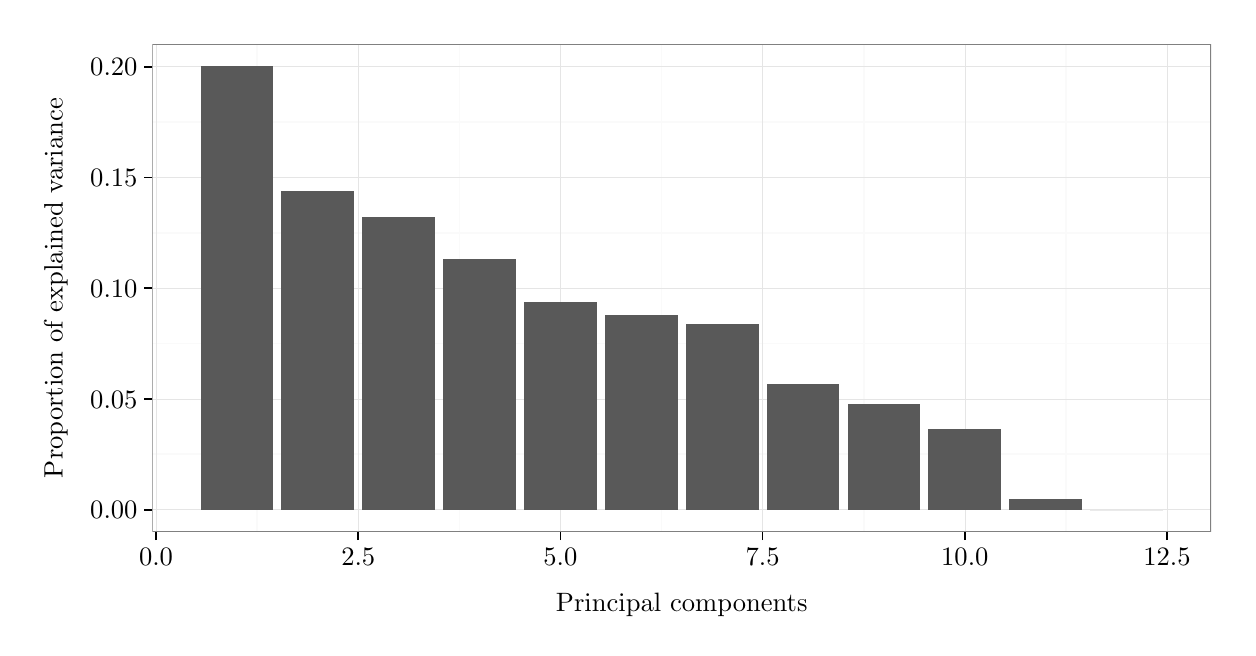
\begin{tikzpicture}[x=1pt,y=1pt]
\definecolor{fillColor}{RGB}{255,255,255}
\path[use as bounding box,fill=fillColor,fill opacity=0.00] (0,0) rectangle (433.62,216.81);
\begin{scope}
\path[clip] (  0.00,  0.00) rectangle (433.62,216.81);
\definecolor{drawColor}{RGB}{255,255,255}
\definecolor{fillColor}{RGB}{255,255,255}

\path[draw=drawColor,line width= 0.6pt,line join=round,line cap=round,fill=fillColor] (  0.00,  0.00) rectangle (433.62,216.81);
\end{scope}
\begin{scope}
\path[clip] ( 45.07, 34.62) rectangle (427.62,210.81);
\definecolor{fillColor}{RGB}{255,255,255}

\path[fill=fillColor] ( 45.07, 34.62) rectangle (427.62,210.81);
\definecolor{drawColor}{gray}{0.98}

\path[draw=drawColor,line width= 0.6pt,line join=round] ( 45.07, 62.64) --
	(427.62, 62.64);

\path[draw=drawColor,line width= 0.6pt,line join=round] ( 45.07,102.66) --
	(427.62,102.66);

\path[draw=drawColor,line width= 0.6pt,line join=round] ( 45.07,142.68) --
	(427.62,142.68);

\path[draw=drawColor,line width= 0.6pt,line join=round] ( 45.07,182.69) --
	(427.62,182.69);

\path[draw=drawColor,line width= 0.6pt,line join=round] ( 82.92, 34.62) --
	( 82.92,210.81);

\path[draw=drawColor,line width= 0.6pt,line join=round] (155.98, 34.62) --
	(155.98,210.81);

\path[draw=drawColor,line width= 0.6pt,line join=round] (229.04, 34.62) --
	(229.04,210.81);

\path[draw=drawColor,line width= 0.6pt,line join=round] (302.10, 34.62) --
	(302.10,210.81);

\path[draw=drawColor,line width= 0.6pt,line join=round] (375.16, 34.62) --
	(375.16,210.81);
\definecolor{drawColor}{gray}{0.90}

\path[draw=drawColor,line width= 0.2pt,line join=round] ( 45.07, 42.63) --
	(427.62, 42.63);

\path[draw=drawColor,line width= 0.2pt,line join=round] ( 45.07, 82.65) --
	(427.62, 82.65);

\path[draw=drawColor,line width= 0.2pt,line join=round] ( 45.07,122.67) --
	(427.62,122.67);

\path[draw=drawColor,line width= 0.2pt,line join=round] ( 45.07,162.69) --
	(427.62,162.69);

\path[draw=drawColor,line width= 0.2pt,line join=round] ( 45.07,202.70) --
	(427.62,202.70);

\path[draw=drawColor,line width= 0.2pt,line join=round] ( 46.39, 34.62) --
	( 46.39,210.81);

\path[draw=drawColor,line width= 0.2pt,line join=round] (119.45, 34.62) --
	(119.45,210.81);

\path[draw=drawColor,line width= 0.2pt,line join=round] (192.51, 34.62) --
	(192.51,210.81);

\path[draw=drawColor,line width= 0.2pt,line join=round] (265.57, 34.62) --
	(265.57,210.81);

\path[draw=drawColor,line width= 0.2pt,line join=round] (338.63, 34.62) --
	(338.63,210.81);

\path[draw=drawColor,line width= 0.2pt,line join=round] (411.69, 34.62) --
	(411.69,210.81);
\definecolor{fillColor}{gray}{0.35}

\path[fill=fillColor] ( 62.46, 42.63) rectangle ( 88.76,202.80);

\path[fill=fillColor] ( 91.69, 42.63) rectangle (117.99,157.79);

\path[fill=fillColor] (120.91, 42.63) rectangle (147.21,148.28);

\path[fill=fillColor] (150.14, 42.63) rectangle (176.44,133.11);

\path[fill=fillColor] (179.36, 42.63) rectangle (205.66,117.57);

\path[fill=fillColor] (208.58, 42.63) rectangle (234.89,112.83);

\path[fill=fillColor] (237.81, 42.63) rectangle (264.11,109.59);

\path[fill=fillColor] (267.03, 42.63) rectangle (293.33, 87.92);

\path[fill=fillColor] (296.26, 42.63) rectangle (322.56, 80.94);

\path[fill=fillColor] (325.48, 42.63) rectangle (351.78, 71.85);

\path[fill=fillColor] (354.71, 42.63) rectangle (381.01, 46.62);

\path[fill=fillColor] (383.93, 42.63) rectangle (410.23, 42.63);
\definecolor{drawColor}{gray}{0.50}

\path[draw=drawColor,line width= 0.6pt,line join=round,line cap=round] ( 45.07, 34.62) rectangle (427.62,210.81);
\end{scope}
\begin{scope}
\path[clip] (  0.00,  0.00) rectangle (433.62,216.81);
\definecolor{drawColor}{RGB}{0,0,0}

\node[text=drawColor,anchor=base east,inner sep=0pt, outer sep=0pt, scale=  0.96] at ( 39.67, 39.33) {0.00};

\node[text=drawColor,anchor=base east,inner sep=0pt, outer sep=0pt, scale=  0.96] at ( 39.67, 79.34) {0.05};

\node[text=drawColor,anchor=base east,inner sep=0pt, outer sep=0pt, scale=  0.96] at ( 39.67,119.36) {0.10};

\node[text=drawColor,anchor=base east,inner sep=0pt, outer sep=0pt, scale=  0.96] at ( 39.67,159.38) {0.15};

\node[text=drawColor,anchor=base east,inner sep=0pt, outer sep=0pt, scale=  0.96] at ( 39.67,199.40) {0.20};
\end{scope}
\begin{scope}
\path[clip] (  0.00,  0.00) rectangle (433.62,216.81);
\definecolor{drawColor}{RGB}{0,0,0}

\path[draw=drawColor,line width= 0.6pt,line join=round] ( 42.07, 42.63) --
	( 45.07, 42.63);

\path[draw=drawColor,line width= 0.6pt,line join=round] ( 42.07, 82.65) --
	( 45.07, 82.65);

\path[draw=drawColor,line width= 0.6pt,line join=round] ( 42.07,122.67) --
	( 45.07,122.67);

\path[draw=drawColor,line width= 0.6pt,line join=round] ( 42.07,162.69) --
	( 45.07,162.69);

\path[draw=drawColor,line width= 0.6pt,line join=round] ( 42.07,202.70) --
	( 45.07,202.70);
\end{scope}
\begin{scope}
\path[clip] (  0.00,  0.00) rectangle (433.62,216.81);
\definecolor{drawColor}{RGB}{0,0,0}

\path[draw=drawColor,line width= 0.6pt,line join=round] ( 46.39, 31.62) --
	( 46.39, 34.62);

\path[draw=drawColor,line width= 0.6pt,line join=round] (119.45, 31.62) --
	(119.45, 34.62);

\path[draw=drawColor,line width= 0.6pt,line join=round] (192.51, 31.62) --
	(192.51, 34.62);

\path[draw=drawColor,line width= 0.6pt,line join=round] (265.57, 31.62) --
	(265.57, 34.62);

\path[draw=drawColor,line width= 0.6pt,line join=round] (338.63, 31.62) --
	(338.63, 34.62);

\path[draw=drawColor,line width= 0.6pt,line join=round] (411.69, 31.62) --
	(411.69, 34.62);
\end{scope}
\begin{scope}
\path[clip] (  0.00,  0.00) rectangle (433.62,216.81);
\definecolor{drawColor}{RGB}{0,0,0}

\node[text=drawColor,anchor=base,inner sep=0pt, outer sep=0pt, scale=  0.96] at ( 46.39, 22.61) {0.0};

\node[text=drawColor,anchor=base,inner sep=0pt, outer sep=0pt, scale=  0.96] at (119.45, 22.61) {2.5};

\node[text=drawColor,anchor=base,inner sep=0pt, outer sep=0pt, scale=  0.96] at (192.51, 22.61) {5.0};

\node[text=drawColor,anchor=base,inner sep=0pt, outer sep=0pt, scale=  0.96] at (265.57, 22.61) {7.5};

\node[text=drawColor,anchor=base,inner sep=0pt, outer sep=0pt, scale=  0.96] at (338.63, 22.61) {10.0};

\node[text=drawColor,anchor=base,inner sep=0pt, outer sep=0pt, scale=  0.96] at (411.69, 22.61) {12.5};
\end{scope}
\begin{scope}
\path[clip] (  0.00,  0.00) rectangle (433.62,216.81);
\definecolor{drawColor}{RGB}{0,0,0}

\node[text=drawColor,anchor=base,inner sep=0pt, outer sep=0pt, scale=  0.96] at (236.35,  6.00) {Principal components};
\end{scope}
\begin{scope}
\path[clip] (  0.00,  0.00) rectangle (433.62,216.81);
\definecolor{drawColor}{RGB}{0,0,0}

\node[text=drawColor,rotate= 90.00,anchor=base,inner sep=0pt, outer sep=0pt, scale=  0.96] at ( 12.61,122.72) {Proportion of explained variance};
\end{scope}
\end{tikzpicture}
